\documentclass[12pt, a4paper]{article}

% Packages and Formatting
\usepackage{../../sub/mystyle_general}
\usepackage{../../sub/mystyle_article}


\title{Lista 1 - Introdução a Análise de Dados \\
Funções \\
Gabarito}
\author{Guilherme Masuko}
\date{March 2023}
%\affil{}

\definecolor{dkgreen}{rgb}{0,0.6,0}
\definecolor{gray}{rgb}{0.5,0.5,0.5}
\definecolor{mauve}{rgb}{0.58,0,0.82}

\lstset{frame=tb,
	language=R,
	aboveskip=3mm,
	belowskip=3mm,
	showstringspaces=false,
	columns=flexible,
	basicstyle={\small\ttfamily},
	numbers=none,
	numberstyle=\tiny\color{gray},
	keywordstyle=\color{blue},
	commentstyle=\color{dkgreen},
	stringstyle=\color{mauve},
	breaklines=true,
	breakatwhitespace=true,
	tabsize=3
}

\lstset{inputencoding=utf8/latin1}


\begin{document}

% Title Page
\clearpage
\maketitle
\thispagestyle{empty}

\textbf{Questão 1}

Crie uma função que recebe três parâmetros $a$, $b$, $c$, os coeficientes de uma função do segundo grau e retorne as raízes dessa função.

Uma função do segundo grau tem a seguinte forma 

\begin{align*}
	f(x) = ax^2 + bx + c
\end{align*}

As raízes de uma função do segundo grau são os $x$'s cujo a função $f(x)$ cruza o eixo das abscissas (horizontal), isso é, $f(x) = 0$.

Para criar a função precisamos relembrar da fórmula de Bhaskara.\footnote{\url{https://pt.wikipedia.org/wiki/F\%C3\%B3rmula_quadr\%C3\%A1tica}}

\begin{align*}
	\Delta &= b^2 -4\cdot a\cdot c \\
	x_{1,2} &= \frac{-b \pm \sqrt{\Delta}}{2\cdot a}
\end{align*}

Lembre-se dos casos em que $\Delta$ é negativo, positivo e igual a zero.

Teste sua função para as seguintes funções:

\begin{itemize}
	\item $f(x) = x^2$
	\item $f(x) = 2x^2 - 18$
	\item $f(x) = x^2 - 4x + 10$
	\item $f(x) = -2x^2 + 20x - 50$
\end{itemize}



\textbf{Solução}

\lstinputlisting[language=R]{codes/solution1.R}




\textbf{Questão 2}

Com base na questão anterior, crie uma nova função que recebe os mesmos parâmetros $a$, $b$ e $c$, coeficientes de uma função do segundo grau, mas que agora retorno um gráfico dessa função.



\textbf{Solução}

\lstinputlisting[language=R]{codes/solution2.R}


Plots resultantes.


\begin{figure}[H]
	\caption{$f(x) = x^2$}
	\centering
	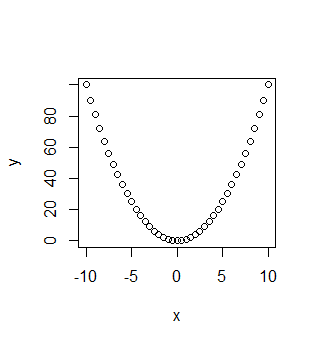
\includegraphics[scale=1]{images/function1.png}
	\label{fig:function1}
\end{figure}

\begin{figure}[H]
	\caption{$f(x) = 2x^2 - 18$}
	\centering
	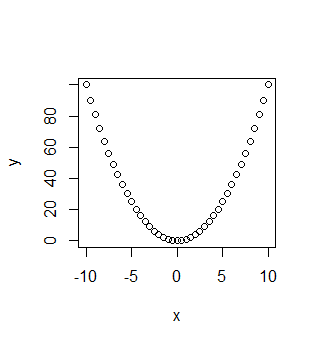
\includegraphics[scale=1]{images/function1.png}
	\label{fig:function2}
\end{figure}


\begin{figure}[H]
	\caption{$f(x) = x^2 - 4x + 10$}
	\centering
	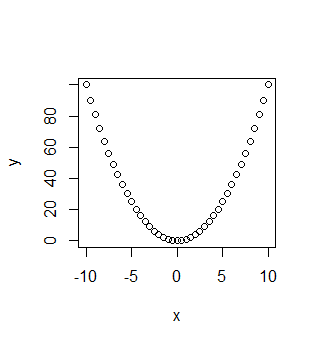
\includegraphics[scale=1]{images/function1.png}
	\label{fig:function3}
\end{figure}


\begin{figure}[H]
	\caption{$f(x) = -2x^2 + 20x - 50$}
	\centering
	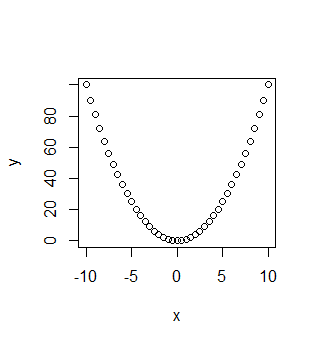
\includegraphics[scale=1]{images/function1.png}
	\label{fig:function4}
\end{figure}




\textbf{Questão 3}

Crie uma função que recebe um número como parâmetro e devolve se o número é primo ou não.

Definição de número primo: Um número primo é um número natural maior que um, tal que não é resultado do produto da multiplicação de dois números naturais, isso é, são números que são divisíveis apenas por ele mesmo dentro da classe dos naturais sem o 1.\footnote{\url{https://pt.wikipedia.org/wiki/Numero_primo}}

Dica: A função que retorna o resto da divisão inteira é '\%\%'.

Teste sua função para os seguintes valores

\begin{itemize}
	\item valores de 2 à 20
	\item 577
	\item 753
	\item 997
\end{itemize}



\textbf{Solução}

\lstinputlisting[language=R]{codes/solution3.R}

	
\end{document}